\section{Token Sequence Normalization}\label{sec:tsn}

In this section, we introduce our first defense mechanism (\contribution{3.1}) called \textit{token sequence normalization}~\cite{Saglam2024b}.
A few years ago, \citet{DevoreMcDonald2020} introduced \textit{\mossad}, a plagiarism generator inspired by genetic programming that allows generating multiple obfuscated versions of a single program.
While most software plagiarism detectors exhibit resilience against some \textit{obfuscation attacks}~\cite{Joy1999,prechelt2000}, \mossad exploits a vulnerability that is inherent in the most widely used approaches.
Although there are graph-based approaches that are potentially less vulnerable to such attacks, they are not feasible in practice~\cite{liu2006} since the subgraph isomorphism problem is NP-complete~\cite{Shang2008, McCreesh2020, Lubiw1981}.

As discussed, \mossad repeatedly inserts statements into the plagiarized program to interfere with the subsequence matching of a potential detector.
To that end, sets of pre-defined statements called \textit{entropy} and existing statements from the original program are used.
The insertion is stopped when the plagiarized instance falls below a certain similarity threshold compared to the original.
%
While \mossad is only one example of an automated obfuscation attack, it is highly effective as similar attacks based on statement insertion are not hard to implement. Thus, it is especially important to provide strong resilience to insertion-based obfuscation.

Token sequence normalization successfully provides resilience against such automatic obfuscation attacks.
It combines the effectiveness of graph-based approaches with the scalability of token-based approaches in a best-of-both-worlds approach\footnote{Subgraph isomorphism for two graphs with $n$ vertices has a runtime complexity of $O(n^n)$. Moreover, the advantage of token sequence normalization is that it has to be performed once per program, not per comparison.}.
We leverage program dependence graphs (PDG)~\cite{ferrante1987} to normalize programs.
However, for real-world applicability, any approach should not be language dependent and operate at an abstract level~\cite{prechelt2002, liu2006, Nichols2019}. Furthermore, it must support explainability via traceability, enabling visualization based on the original, unaltered code.
From both ethical and administrative standpoints~\cite{Simon2016, Le2013}, only the original, unaltered code should inform human decision-making in academic misconduct investigations.
Moreover, the unaltered code often contains idiosyncrasies~\cite{Novak2019} due to obfuscation. They are used for both initial decision-making and misconduct investigations.
Hence, it is not sufficient to eliminate dead code in the input programs.
Existing dead code elimination methods do not fulfill these requirements, as they are fully language-dependent, modify the programs, and are incompatible with ethical and administrative concerns.

In contrast to dead code elimination, our defense mechanism is specifically designed to meet these requirements.
It expands upon the inherent resilience of token-based approaches by making the token sequence virtually invariant against insertion- and reordering-based attacks.
As part of that, we introduce the concept of a \textit{token normalization graph} (TNG), which operates on the token sequence and is thus language-independent.
With that token normalization graph, we normalize the token sequence by removing dead statements and putting subsequent independent statements in a fixed order.
Thus, we effectively reverse the insertion and reordering of statements and de-obfuscate plagiarism instances, thereby achieving high resilience to automatic plagiarism based on these attacks.

\begin{factsheet}{Overview: Token Sequence Normalization} 
    \begin{description}[style=multiline,leftmargin=5.5cm]
        \item[Core Principle] Normalize Token Sequence \\via Graph-Based Representation
        \item[Targeted Obfuscation Attack] Statement Insertion, Statement Reordering
        \item[Language Family] Programming Languages
        \item[Language Dependence] Language-Agnostic
        \item[Performance Impact] Low
        \item[Main Scalability Determinant] Size of Input Programs 
        \item[Integration Complexity] Moderate
    \end{description}
\end{factsheet}

\subsection{Targeted Obfuscation Attacks} \label{sec:icseb:RunningExample}

Token sequence normalization is designed to defend against two particular obfuscation attack types: Semantic-preserving statement insertion and statement reordering. These attacks aim to affect the token sequence derived from a program by modifying the program without changing its underlying behavior, thereby misleading plagiarism detection tools. %Two primary forms of targeted obfuscation attacks are considered: reordering of independent statements and insertion of (dead) statements.

%\subsubsection{Insertion of (Dead) Statements}
A simple yet effective obfuscation attack is the insertion of dead statements. Dead statements are lines of code that do not affect the program's output or behavior. These can include redundant assignments, unused variables, or code blocks that are never executed (e.g., due to always-false conditions). An attacker can significantly alter the token sequence without changing the program's functionality by inserting such statements at various points in the code. Furthermore, dead statements can be obfuscated themselves by inserting further statements that depend on them.

\begin{samepage}
\begin{lstlisting}[caption={Example for Obfuscated Dead Statements},label=lst:complexinsertion]
int x = 10;
boolean checked = false; // Dead statement
int y = 5;
if (checked) { // Dead block, only depends on the dead statement
    y = 20;
}
println(x + y);
\end{lstlisting}
\end{samepage}

\autoref{lst:complexinsertion} illustrates such a dependence between inserted statements. Both the variable \texttt{checked} and the control structure are dead code. However, the variable is referenced as a condition of the control structure.
However, as these statements do not alter the behavior of the program, they are still dead code. However, it is harder to detect them, as statement interdependence has to be fully resolved.

%\subsubsection{Reordering of Independent Statements}
Reordering independent statements involves changing the order of code statements that do not depend on each other, meaning the order of the statements does not affect the behavior of the program. This type of obfuscation leverages the fact that most programming languages allow statements that do not affect each other's execution order to be rearranged. For example, swapping the order of two variable assignments that do not depend on each other's values is possible. This attack is considered a weak form of obfuscation, as the degree of freedom to reorder statements in most programs is limited. Only some statements can be reordered, thus making it challenging to apply this obfuscation broadly.

Both statement insertion and reordering can be automated in different ways. Our defense mechanism is designed to counter these attacks independent of their automation, be it \mossad-style random obfuscation until a certain threshold is reached or exhaustive obfuscation where the obfuscation is applied to all possible code positions.

\noindent
As a combined running example for both insertion and reordering, we introduce the programs shown in \autoref{tab:codesnippet}. 
Both programs print the squared values of the numbers from 1 to 10.
The right program is a modified variant based on two changes that alter its structure.
Thus, the program still behaves the same upon execution.
In detail, line 3 was inserted in the modified variant, and lines 6 and 7 were swapped.
%Minimal example, no focus on renaming as popular code plagiarism detectors are resilient by using abstraction \cite{} 
%Also, there is no focus on deletion, as it is not practical if functionality should not be reduced
While the relationship between the programs is evident in this simple example, this is not true for larger programs that undergo extensive modifications to obfuscate the relation between the variant and the original. Thus, these modifications can be used to conceal plagiarism. 
Additionally, manual comparison becomes infeasible when dealing with numerous student submissions, even for smaller programs.
However, for plagiarism detectors, structural obfuscation attacks like these diminish the detection quality~\cite{DevoreMcDonald2020}. 
%Easy to detect, but only minimal example. Large-scale obfuscation in thousands of lines with hundreds of submissions, easy to be overlooked

To illustrate this, \autoref{tab:tokens} shows the token sequences of the two programs in \autoref{tab:codesnippet}.
While the structural information concerning method context, loop context, declarations, and assignments remains intact, specific details such as names, types, or comments are excluded.
Note that the changes lead to two sequences that are different enough to affect the detection quality, as only shorter subsequences can be matched between them. In detail, we can find three matching subsequences of length two: The first two lines, the last two lines, and finally, lines four and five. As discussed, these subsequences are short enough to fall below the plagiarism detector's threshold.

\begin{samepage}
\begin{table}
	\centering
	\begin{tabular}{rlcl}
		\toprule
		\textbf{\#} & \textbf{Original}                              &                  & \textbf{Variant}                                   \\
		\midrule
		1           & \texttt{~~void printSquares() \{}              &                                    & \texttt{~~void printSquares() \{}                  \\
		2           & \texttt{~~~~int i = 1;}                        &                                    & \texttt{~~~~int i = 1;}                            \\
				
		3           &                                                & \small\textbf{\phantom{$\to$}  insert $\to$} & \cellcolor{add}\texttt{~~~~boolean debug = false;} \\
				
		4           & \texttt{~~~~while (i <= 10) \{}                &                                    & \texttt{~~~~while (i <= 10) \{}                    \\
		5           & \texttt{~~~~~~int square = i * i;}             &                                    & \texttt{~~~~~~int square = i * i;}                 \\
		6           & \cellcolor{del}\texttt{~~~~~~println(square);} & \small\textbf{$\to$ reorder $\to$} & \cellcolor{add} \texttt{~~~~~~i++;}                \\
		7           & \cellcolor{del}\texttt{~~~~~~i++;}             & \small\textbf{$\to$ reorder $\to$} & \cellcolor{add} \texttt{~~~~~~println(square);}    \\
		8           & \texttt{~~~~\}}                                &                                    & \texttt{~~~~\}}                                    \\
		9           & \texttt{~~\}}                                  &                                    & \texttt{~~\}}                                      \\
		\bottomrule
	\end{tabular}
    \caption[Example Obfuscation: Insertion and Reordering]{Original code (left) and modified variant (right) after inserting one statement and reordering two. Removed lines are highlighted in red, and added lines are highlighted in green.}
	\label{tab:codesnippet}
\end{table}


\begin{table}
    \centering
    %\small
    \begin{tabular}{c@{\hskip 15pt}l@{\hskip 30pt}c@{\hskip 30pt} r}
        \toprule
        \# & \textbf{Original Tokens}     &                     & \textbf{Variant Tokens}      \\
        \midrule
        1  & \texttt{method start} &                 & \texttt{method start} \\
        2  & \texttt{variable}     &                 & \texttt{variable}     \\
        3  &                       & \textbf{\phantom{$\to$}  insert $\to$}    & \cellcolor{add}\texttt{variable}     \\
        4  & \texttt{loop start}   &                 & \texttt{loop start}   \\
        5  & \texttt{variable}     &                 & \texttt{variable}     \\
        6  & \cellcolor{del}\texttt{apply}        & \textbf{$\to$  swap $\to$} & \cellcolor{add}\texttt{assignment}   \\
        7  & \cellcolor{del}\texttt{assignment}   & \textbf{$\to$  swap $\to$} & \cellcolor{add}\texttt{apply}        \\
        8  & \texttt{loop end}     &                 & \texttt{loop end}     \\
        9  & \texttt{method end}   &                 & \texttt{method end}   \\
        \bottomrule
    \end{tabular}
    \caption[Example Obfuscation Tokens: Insertion and Reordering]{Comparison of the original and obfuscated token sequences corresponding to the program statements in \autoref{tab:codesnippet}. One token is inserted at index 3, while two tokens at indices 6 and 7 are swapped.}
    \label{tab:tokens}
\end{table}
\end{samepage}

\subsection{Concept}

The defense mechanism is an additional step in the pipeline of a plagiarism detector before the pairwise comparison, which effectively de-obfuscates plagiarism for the remaining steps in the pipeline.
At a high level, our mechanism operates as follows for each input program:

\begin{enumerate}
    \item We enrich the token sequence with additional language-agnostic semantic information about the interdependence of the tokens.
    \item We construct a language-independent graph-based representation of the tokenized program from the enriched token sequence, which abstracts from the original code. This graph represents a partial order of the tokens.
    \item We then use this graph to generate a normalized token sequence, thus effectively reverting insertions and reordering operations.
    \begin{enumerate}
        \item Insertions are countered via subsequence removal.
        \item Reordering is negated by topological sorting~\cite{kahn1962}.
    \end{enumerate}
    \item The comparison is still conducted exclusively on the token sequence, circumventing the computational complexity of graph-based approaches.
\end{enumerate}

\noindent
We call the representation of the tokenized program a \textit{token normalization graph} (TNG).
Each node in this graph represents the tokens of a program statement.
As it is based on the token sequence, it is language-independent, which enables our defense mechanism to be applicable to any programming language.
Thus, the format of the semantic information utilized to enrich the token sequence must also be language-independent.
%
We specify a generic format for the semantic information based on the interdependence between tokens that abstracts from the detail of the underlying programming language.
The semantic information must be extracted from the input programs alongside the tokens.
Therefore, the extraction needs to be implemented separately for each language the detector supports.
It is the sole language-dependent step that our defense mechanism adds.
While the format of the semantic information and the TNG is language-independent, the need to provide this information makes the defense mechanism language-agnostic.
However, extracting semantic information does not impose additional constraints on the detector since tokenization is inherently language-dependent.


\subsection{Semantic Information}

\label{subsec:semantic}
In order to construct a TNG, we need information about the interdependencies between the tokens.
This information is not present in the token sequence and thus must be additionally attached to the tokens.
To that end, a language-independent format is required for this semantic information.
Using this format, the tokens can be automatically annotated during their extraction from the parse tree. Different types of statements lead to different types of information.
Thus, this format allows us to map the relations of the statements in the program to the tokens independent of the underlying language of the program.
%
We specify the following format for this semantic information:
%\begin{samepage}
\begin{description}
    \item[Criticality] describes statements that contribute to programs' behavior through means other than variables and thus must not be removed. Therefore, a token can be either critical or not critical.
        \textit{In our example in \autoref{tab:codesnippet}, the critical statements are the \texttt{while} statement and the \texttt{println} statement. Thus, the \texttt{loop start} and \texttt{apply} tokens in \autoref{tab:tokens} are critical.}
    \item[Fixed Order] describes how statements must maintain their relative order to ensure semantic equivalence. Tokens can thus be either fixed in their order or non-fixed. Fixed order tokens act as reordering boundary, as preceding tokens cannot be moved after this boundary and vice versa.
        \textit{In the running example, the \texttt{while} statement dictates that the statements within the loop cannot be moved outside the loop. Thus, the loop tokens of lines 4 and 8 in \autoref{tab:tokens} are fixed order tokens.}
    \item[Variable Access] describes the variable accesses (read or write) for each statement, thus indicating on which other statements they depend.
        Hence, each token has two variable identifier sets: One for read accesses and one for write accesses.
        \textit{In the running example, the \texttt{while} statement depends on the statement the declares the variable \texttt{i}. Therefore, the \texttt{loop start} token contains \texttt{i} in its read access set.}
    \item[Loop] describes statement blocks in which the execution order of the statements can deviate from their declaration order. Therefore, the first and last tokens corresponding to the loop are marked with loop start and loop end flags.
        \textit{In the running example, the statements in the loop body are repeatedly executed. Thus, the incrementation of the variable \texttt{i} may be executed not only after the \texttt{println} statement but also before due to the repeated execution. In the running example, both \texttt{loop start} and \texttt{loop end} are marked with the loop flag.}
\end{description}
%\end{samepage}


\subsection{Token Normalization Graph}

We use the token normalization graph (TNG) as the underlying data structure to generate a normalized token sequence.
A TNG is a specialized version of a program dependence graph (PDG).
It is designed for tokens instead of code and through a higher abstraction level not confined to the programming language's syntax. Thus, a TNG crucially provides language independence. A TNG contains additional edges required for the token sequence normalization.
While a PDG focuses only on statement dependencies in code, the TNG considers both token interdependence and the order of the tokens. Both are required for token-based approaches.

We construct the TNG from the token sequence and the additional semantic information.
A TNG node represents a single statement and contains all tokens generated from that statement.
After the construction of the TNG, we no longer need the original token sequence.
%
More formally, a token normalization graph is a directed graph \( G = (V, E) \) used to represent the tokenized form of a program for the purpose of normalization. Each node \( v \in V \) represents a statement in the program and contains a subsequence of tokens. Let \( (t_i) \) be the sequence of all tokens in the program. Each statement \( S \) corresponds to a subsequence \( (s_j) \sqsubseteq (t_i) \) where \( (s_j) \) is the set of tokens extracted for \( S \). Thus, each node in the TNG is represented by a subsequence of tokens.
%
The TNG has three types of directed edges, each capturing different dependencies between the statements represented by the nodes:
\begin{description}
    \item[Variable Flow Edges] indicate that a statement writes to a variable that another statement reads. They are similar to the data dependencies in the PDG.
    \textit{A directed edge \( (v_i, v_j) \in E \) is a variable flow edge $(v_i, v_j) \in E_{vf}$ if statement \( S_i \) of $v_i$ writes to a variable that statement \( S_j \) of $v_j$  reads. This edge indicates a data dependency where \( v_j \) depends on \( v_i \) for the value of the variable.}
    
    \item[Variable Order Edges] indicate that altering the order of the two statements may alter variable values and, thus, the program's behavior.
    This edge helps maintain the correct execution order of statements.
    Wherever there is a variable flow edge, there is also a variable order edge; however, not necessarily in the same direction.
     \textit{A directed edge \( (v_i, v_j) \in E \) is a variable order edge $(v_i, v_j) \in E_{vo}$ if changing the relative order of statements \( S_i \) and \( S_j \) could alter the program's behavior due to variable dependencies.}
     
    \item[Fixed Order Edges] indicate that altering the order of the two statements may affect the program's behavior for reasons beyond variable value alterations.
    This edge enforces the preservation of the original order of critical statements.
    \textit{A directed edge \( (v_i, v_j) \in E \) is a fixed order edge $(v_i, v_j) \in E_{fo}$ if changing the order of statements \( S_i \) and \( S_j \) could affect the program's behavior for reasons other than variable dependencies.}   
\end{description}

\noindent
The TNG is then constructed as follows:
First, we group all tokens within a statement as nodes. %, and edges are then formed based on the tokens' semantic information.
For each statement \( S \) in the program, create a node \( v_i \) containing the subsequence of tokens \( (s_j) \sqsubseteq (t_i) \).
Next, we label nodes containing at least one critical token as \textit{critical}.
We then use the tokens marked as \textit{fixed order} to create fixed order edges $E_{fo}$.
For each node with fixed order tokens, we create incoming and outgoing edges to and from all preceding and subsequent nodes, as determined by the original order of the tokens.
We employ the variable access sets and loop flags to create variable flow edges $E_{vf}$.
Finally, disregarding loop flags, we determine variable order edges $E_{vo}$ solely by variable access sets.
Once the TNG is complete, it contains all the necessary data for generating a normalized token sequence. Thus, the original token sequences can be safely discarded.
Moreover, as for all token-based approaches, the original programs are no longer required for the similarity calculation.


\begin{figure}
\centering
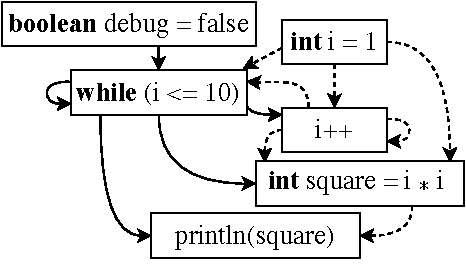
\includegraphics[width=0.5\linewidth]{figures/pdg.pdf}
\caption[Program Dependence Graph]{Program dependence graph of the running example showing control dependencies (solid arrows) and data dependencies (dashed arrows).}
\label{fig:pdg}
\end{figure}


\autoref{fig:pdg} shows a PDG for the plagiarized program in \autoref{tab:codesnippet}. The control and data dependencies between the different code statements are represented via edges.
While the dead statement for the variable called \texttt{debug} can be identified, it cannot be used to generate a normalized token sequence due to the requirements mentioned in \autoref{sec:tsn-requirements}.
\autoref{fig:tng} shows the TNG for the same program. In contrast to the PDG, the nodes represent tokens instead of code. The TNG contains the three types of edges based on the semantic information discussed in \autoref{subsec:semantic}. The two nodes with a gray background are marked as critical. Furthermore, the semantic information of the corresponding tokens is illustrated in the bottom right corner of the node. 
The semantic information is only depicted for the sake of clarity. It is used to construct the TNG but is no longer necessary for the normalization thereafter.

\begin{figure}
\centering
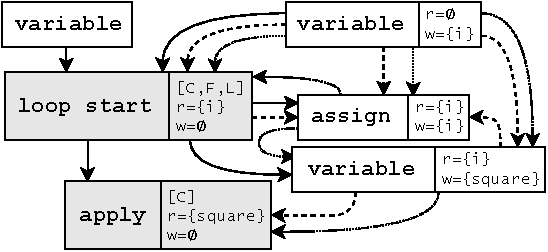
\includegraphics[width=0.6\linewidth]{figures/tng3.pdf}
\caption[Token Normalization Graph]{Token normalization graph for the PDG in \autoref{fig:pdg}, fixed order edges (solid), variable order edges (dashed), and variable flow edges (dotted).
The critical (C), fixed-order (F), and loop (L) flags, with the variable access sets (r for read, w for write), are included for illustrative purposes.}
\label{fig:tng}
\end{figure}


\subsection{Generating the Normalized Token Sequence}

After constructing the TNG, we can leverage it to generate a normalized token sequence in two steps.
%We do so in two steps: One for reverting insertions and one for reverting reordering.
First, we remove all dead nodes. These are all nodes from which no critical node can be reached via variable flow edges $E_{vf}$. This effectively reverts insertions into the token sequence.
Next, we remove all variable flow edges $E_{vf}$ from the TNG, making it acyclical. They have served their purpose for the dead node removal and are no longer required.
In our running example in \autoref{tab:codesnippet}, the statement containing the variable named \texttt{debug} is considered dead code, and so is its corresponding \texttt{variable} node in the TNG in \autoref{fig:tng}.
This node will be removed, as it has no outgoing variable flow edge.
\autoref{tab:tokens-full} illustrates how that affects the normalized token sequence. The code insertion leads to an additional token in the obfuscated token sequence. However, after the dead node removal, this effect is reversed.
\autoref{fig:tng2} illustrates the TNG from \autoref{fig:tng} with the dead node removed and variable flow edges $E_{vf}$ omitted. The previous cycles, such as the one between the \texttt{loop start} and \texttt{assign} nodes, are no longer present.
A partial order becomes apparent when considering the topmost \texttt{variable} node as the root.

\begin{figure}[b]
\centering
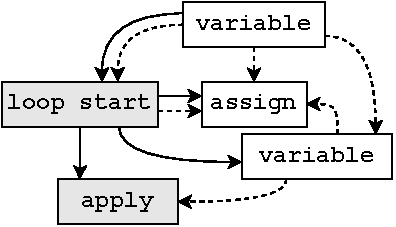
\includegraphics[width=0.45\linewidth]{figures/tng2b.pdf}
\caption[Reduced Token Normalization Graph]{Token normalization graph after the dead nodes and removal of variable flow edges, still present are fixed order edges (solid) and variable order edges (dashed).}
\label{fig:tng2}
\end{figure}

Next, we use topological sorting~\cite{kahn1962} to generate a normalized token sequence. This counters attempts to reorder the token sequence.
Specifically, we order the tokens of the remaining nodes by their node's distance to the aforementioned root.
Nodes with the same distance represent subsequent independent statements. We sort them via the types of tokens in the nodes.
This is a robust criterion, as the extracted tokens are invariant to lexical modifications~\cite{prechelt2002}.
Note that if two nodes with the same root distance are equal according to that criterion, they contain the same tokens, and their order does not affect the normalized token sequence. %; therefore, we can consider them equal in order.

In our running example in \autoref{tab:codesnippet}, statements 6 and 7 were swapped.
\autoref{tab:tokens-full} illustrates how this obfuscation affects the token sequence.
When using the reduced TNG in \autoref{fig:tng2} to generate the normalized token sequence, the sequence after the topological sorting will be identical to the original one (see \autoref{tab:tokens-full}). Thus, the plagiarism detector computes a 100\% match for our running example, despite the obfuscation attempt shown in \autoref{tab:codesnippet}.
Our approach only normalizes the tokens sequence. The original, unaltered code, with all its idiosyncrasies, is used for the visualization. However, as a result of our normalization, the similarity calculation and code matching are not compromised by obfuscation attacks.




\begin{table}
    \centering
    \begin{tabular}{c@{\hskip 12pt}c@{\hskip 4pt}c@{\hskip 4pt}c@{\hskip 4pt}c@{\hskip 4pt}c@{\hskip 4pt}c@{\hskip 4pt}c}
        \toprule
        \# & \textbf{Original} & $\to$ & \textbf{Obfuscated} & $\to$ & \textbf{Nodes Removed} & $\to$ & \textbf{Top. Sorted} \\
        \midrule
        {1}  & \texttt{method start} & & \texttt{method start} & & \texttt{method start} & & \texttt{method start} \\
        {2}  & \texttt{variable}     & & \texttt{variable}     & & \texttt{variable}     & & \texttt{variable}     \\
        {3}  &                                  & \textbf{(+)} & \texttt{\textbf{variable}}     & \textbf{(--)} & & &  \\
        {4}  & \texttt{loop start}   & & \texttt{loop start}   & & \texttt{loop start}   & & \texttt{loop start}   \\
        {5}  & \texttt{variable}     & & \texttt{variable}     & & \texttt{variable}     & & \texttt{variable}     \\
        {6}  & \texttt{apply}        & \textbf{(\textasciitilde)} & \texttt{\textbf{assignment}}   & & \texttt{\textbf{assignment}}   & \textbf{(\textasciitilde)}& \texttt{apply}   \\
        {7}  & \texttt{assignment}   & \textbf{(\textasciitilde)} & \texttt{\textbf{apply}}        & & \texttt{\textbf{apply}}        & \textbf{(\textasciitilde)}& \texttt{assignment}        \\
        {8}  & \texttt{loop end}     & & \texttt{loop end}     & & \texttt{loop end}     & & \texttt{loop end}     \\
        {9}  & \texttt{method end}   & & \texttt{method end}   & & \texttt{method end}   & & \texttt{method end}   \\
        \bottomrule
    \end{tabular}
    \caption[Token Sequence Normalization]{Comparison of the original and obfuscated token sequences with the obfuscated one after the two steps dead node removal and topological sorting \autoref{tab:codesnippet}.}
    \label{tab:tokens-full}
\end{table}


\subsection{Complexity}

The runtime complexity of token sequence normalization depends on extracting the semantic information, creating the token normalization graph, and generating the normalized token sequence.
The semantic information can be extracted during the tokenization step of the plagiarism detector and does not occur at an additional cost.

For the other steps, the runtime complexity depends on the density of the graph and, thus, on its number of nodes, which is limited by the number of tokens $m$ and its number of edges $e$.
As for a PDG, building a TNG can take $O(m^2)$ time in the worst case due to dense dependencies among tokens.
Pruning dead nodes requires a reachability analysis using a graph traversal with a $O(m + e)$ complexity. Topological sorting is performed on the resulting TNG and takes $O(m + e)$ time.

Therefore, the overall runtime complexity is $O(m^2)$ in the worst case (for dense graphs) and $O(m + e)$ in the best case (for sparse graphs).
Note that this has to be done for every input program but not for every comparison, which is a strong advantage compared to graph-based plagiarism detection methods. Thus, doing so for $n$ programs of maximum $m$ tokens has a worst-case complexity of only $O(nm^2)$. Thus, the size of the input programs has a larger impact on the performance of the token sequence normalization than the number of programs.
%
As the worst-case runtime complexity for greedy string tiling for $n$ programs with $m$ tokens, each is \( O(n^2m^3) \) (see \autoref{sec:found-jplag}), token sequence normalization does not increase the runtime complexity of the plagiarism detection process.


\subsection{Observed Impact}
This section presents initial observations on the effectiveness of token sequence normalization based on real-world data. It is important to note that this is not intended as a comprehensive evaluation but instead aims to provide an empirical perspective on how the defense mechanism performs in practical scenarios.

When applying token sequence normalization in practice, we can observe that it effectively renders obfuscation attacks based on insertion and reordering ineffective.
Remarkably, the similarity of unrelated solutions remains virtually unaltered, with an average similarity increase of less than 1\%, effectively avoiding an increase in false positives.
Our defense mechanism comes with a negligible runtime overhead of mere seconds for large real-world datasets, thus showing its practicality.

\autoref{fig:tsn-impact} illustrated the effectiveness of our approach in preventing obfuscation statement insertion.
The solid lines show how the similarity computed by JPlag decreases the more statements proportionally to the input program size are inserted.
Without our defense mechanism, the similarity values drop below 10\%. This renders successful plagiarism detection ineffective, as plagiarized programs can no longer be distinguished from original ones.
To achieve such a low threshold, approximately 50-60\% additional statements need to be inserted.
Note that we employed PlagGen~\cite{Broedel2023} for the obfuscation, which uses an exhaustive strategy. Thus, the input program determines how many statements can be inserted. 

The dashed lines show the same input programs but with token sequence normalization enabled. 
There, the similarity values surge to over 99\%. These results would raise strong suspicions, as for its dataset, the average similarity of unrelated programs is around 10\%. Thus, token sequence normalization renders the obfuscation attack ineffective, making the detector resilient against these attacks.

\begin{figure}[ht]
    \centering
    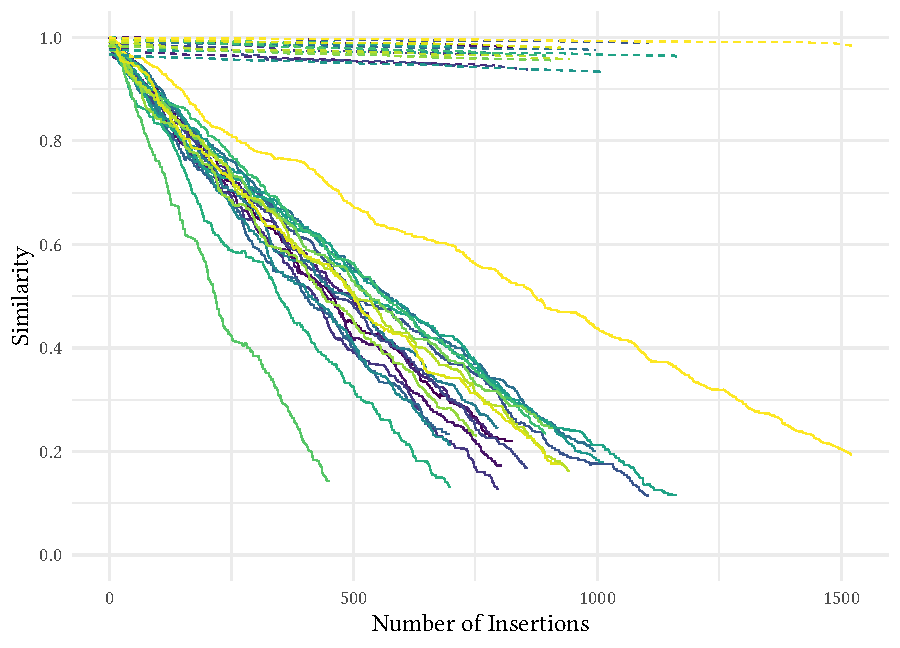
\includegraphics[width=1\linewidth]{figures/eval-tsn-steps.pdf}
    \caption[Impact of Token Sequence Normalization]{Similarities calculated by JPlag for obfuscated programs of a real-world introductory programming assignment dataset with an average of 1529 lines of code (LOC) per program via step-wise statement insertion as obfuscation attack. Each line represents a program, solid lines for JPlag as the baseline, and dashed lines are for JPlag with token sequence normalization.}
    \label{fig:tsn-impact}
\end{figure}

To assess the performance implications of our mechanism, we compared the runtime of JPlag with and without our approach.
We measured the runtime for two real-world datasets. We employed a consumer notebook, specifically a MacBook Pro equipped with an M1 Pro chip and 16GB of memory, for our performance measurements to provide a realistic environment.
As shown in \autoref{fig:tsn-runtime}, there is only an overhead of 0.89 seconds for one dataset and 6.45 seconds for the other. Note that this is the overhead for the complete datasets, not individual programs. State-of-the-art software plagiarism detectors like JPlag are highly optimized, and the performance impact of our mechanism is negligible. Thus, the total runtime of JPlag combined with our mechanism is mere seconds.

    \begin{table}
	\centering
	\begin{tabular}{llrrr}
		\toprule
		  Dataset Name & Metric     & JPlag     & JPlag with TSN & Difference\\
		\midrule
		\multirow{ 2}{*}{TicTacToe} & Runtime    & 6.97s     &    7.86s   & +0.89s\\
        %         &Relative Runtime   & 100.0\% &    112.7\% &\\ % with exact measurements it's . 7
	               &  $\sigma$ (SD)    & 0.10s     &    0.10s &+0.00s\\
        \hline 
        \multirow{ 2}{*}{BoardGame}   & Runtime          & 16.83s     &    23.28s   & +6.45s\\
		              & $\sigma$ (SD)    & 0.53s      &    0.44s    & -0.09s \\
		\bottomrule
    \end{tabular}
    \caption[Runtime Overhead of Token Sequence Normalization]{Runtime overhead of JPlag with token sequence normalization for two introductory programming assignment dataset TicTacToe (626 programs, 167.562 LOC total, \textasciitilde200.000 comparisons) and BoardGame (434 programs, 685.730 LOC total, \textasciitilde94.000 comparisons), avg. of 100 runs.}
	\label{fig:tsn-runtime}
    \end{table}
    

\subsection{Limitations}\label{sec:tsn-limits}

While token sequence normalization is a highly effective defense mechanism against insertion-based obfuscation attacks, it does have certain limitations. In the following, we discuss its dependence on the quality of the extracted semantic information and its applicability to other programming paradigms.

\subsubsection{Dependence on Semantic Information Extraction}
Token sequence normalization requires accurate extraction of semantic information during the tokenization step of the plagiarism detector. This semantic information, such as dependencies between tokens, is used to construct the token normalization graph. As previously discussed, this extraction process introduces a small degree of language dependence, as it must be tailored to capture critical relationships within the syntax and semantics of each programming language.
%
Although token sequence normalization overall is language-agnostic in its core design, its effectiveness depends on the quality and accuracy of this language-specific semantic information. We employ a conservative approach and thus only normalize the parts of the token sequence where tokens can be safely reordered or removed, making over-normalization not a problem as long as the extracted semantic information is correct.

However, if not enough semantic information is extracted, for example, only for some program elements, then the effectiveness of the defense mechanism decreases. This does not reduce the overall detection quality; it just reduces the resilience against insertion-based obfuscation attacks. As an example, consider the language C++. For this language, the standards include several cases of undefined behavior. Furthermore, various syntactical variations can express the same program behavior. Finally, its syntax is generally considered very complex.

These aspects make it hard to cover all edge cases when designing the extraction of semantic information for a new language such as C++. The overlooked edge cases could then be exploited to reduce the effectiveness of the defense mechanism, allowing, for example, the insertion of certain dead statements that are not recognized as such.
%
However, even if some edge cases are overlooked, token sequence normalization will still provide significant resilience, thus making effective obfuscation challenging.

\subsubsection{Applicability for Other Language Paradigms}
While the approach for token sequence normalization is language agnostic, applying it to vastly different paradigms, such as purely functional programming languages, presents unique challenges. For languages like Haskell, statement inter-dependencies and control flow differ significantly from languages like Java, C++, or Python.

In functional languages, especially in pure functional ones like Haskell, there are no traditional control flow statements (e.g., loops or conditionals in the imperative sense) that token sequence normalization typically handles through dependency graphs. Functional programs often rely on recursive function calls and higher-order functions, which make token-based sequence normalization less straightforward since there are no explicit control structures to anchor the ordering of the token normalization graph.
%
Moreover, functional languages emphasize immutability and avoid side effects, so they do not use variable assignments or mutable state as imperative languages do. The dependency relationships that token sequence normalization relies on, such as variable flow edges $E_{vf}$ or variable order edges $E_{vo}$, would have limited or no applicability. Haskell, for example, uses function compositions, pure functions, and monads to handle effects and dependencies.
%
Additionally, token sequence normalization is designed to work on a statement-by-statement basis, but functional languages often treat functions or expressions as atomic units. For instance, Haskell functions are typically small, pure, and composable, and their order can frequently be rearranged without affecting program semantics. Thus, a token-based normalization approach, like token sequence normalization, must define meaningful reordering boundaries.

However, this limitation is a broader problem, as plagiarism detection support for functional languages is generally limited~\cite{Hage2013}. However, token sequence normalization applies to the most frequently taught programming languages and thus covers typical use cases for source code plagiarism detection (see \autoref{sec:survey}).

% -------------------------------------------------------------------
\endinput % EVERYTHING BELOW IS EXCLUDED!!!

\begin{table}
    \centering
    \caption{Comparison of the original and obfuscated token sequences with the obfuscated one after the two steps dead node removal and topological sorting \autoref{tab:codesnippet}.}
    \label{tab:tokensfull}
    \scriptsize
    \begin{tabular}{ccccc}
        \hline
        \# & \textbf{Original} & \textbf{Obfuscated} & \textbf{DN Removed} & \textbf{Top. Sorted} \\
        \hline
        1  & \scriptsize\texttt{method start} & \scriptsize\texttt{method start} & \scriptsize\texttt{method start} & \scriptsize\texttt{method start} \\
        2  & \scriptsize\texttt{variable}     & \scriptsize\texttt{variable}     & \scriptsize\texttt{variable}     & \scriptsize\texttt{variable}     \\
        3  &                                  & \scriptsize\texttt{\textbf{variable}}     &                                  &                                   \\
        4  & \scriptsize\texttt{loop start}   & \scriptsize\texttt{loop start}   & \scriptsize\texttt{loop start}   & \scriptsize\texttt{loop start}   \\
        5  & \scriptsize\texttt{variable}     & \scriptsize\texttt{variable}     & \scriptsize\texttt{variable}     & \scriptsize\texttt{variable}     \\
        6  & \scriptsize\texttt{apply}        & \scriptsize\texttt{\textbf{assignment}}   & \scriptsize\texttt{\textbf{assignment}}   & \scriptsize\texttt{apply}   \\
        7  & \scriptsize\texttt{assignment}   & \scriptsize\texttt{\textbf{apply}}        & \scriptsize\texttt{\textbf{apply}}        & \scriptsize\texttt{assignment}        \\
        8  & \scriptsize\texttt{loop end}     & \scriptsize\texttt{loop end}     & \scriptsize\texttt{loop end}     & \scriptsize\texttt{loop end}     \\
        9  & \scriptsize\texttt{method end}   & \scriptsize\texttt{method end}   & \scriptsize\texttt{method end}   & \scriptsize\texttt{method end}   \\
        \hline
    \end{tabular}
\end{table}